\documentclass[conference,a4paper]{IEEEtran}
\ifdefined\pdfminorversion
\pdfminorversion=6
\fi
\renewcommand{\dbltopfraction}{0.95}
\renewcommand{\dblfloatpagefraction}{0.85}
\setcounter{dbltopnumber}{3}

\usepackage{cite}
\usepackage{amsmath,amssymb}
\usepackage{graphicx}
\usepackage{booktabs}
\usepackage{array}
\usepackage{url}
\usepackage{xcolor}
\usepackage{placeins}

\setlength{\textfloatsep}{7pt plus 1.0pt minus 2.0pt}
\setlength{\floatsep}{6pt plus 1.0pt minus 2.0pt}
\setlength{\intextsep}{6pt plus 1.0pt minus 2.0pt}
\setlength{\dbltextfloatsep}{7pt plus 1.0pt minus 2.0pt}
\setlength{\dblfloatsep}{6pt plus 1.0pt minus 2.0pt}
\setlength{\abovecaptionskip}{3pt}
\setlength{\belowcaptionskip}{2pt}
\setlength{\abovedisplayskip}{3pt plus 1.0pt minus 1.0pt}
\setlength{\belowdisplayskip}{3pt plus 1.0pt minus 1.0pt}

\graphicspath{{improve_behavioral_final_results/}{improve_behavioral_final_results/report_outputs/}}

\begin{document}

% \title{Behavior-Aware Multimodal Fusion and Stimulus-Set Optimization for Schizophrenia Recognition from Eye Movements}
\title{BAMF: Behavior-Aware Multimodal Fusion for Schizophrenia Recognition from Eye Movements}

% TODO before submission: confirm author order, affiliations, ORCID identifiers,
% corresponding author, and the official RIVF 2026 template/page limit.
\author{
\IEEEauthorblockN{Duc Minh Vu, Minh Huy Nguyen, Danh Tuan Dung Pham, Hanh Trang Bui, Thanh Hai Tran}
\IEEEauthorblockA{
School of Electrical and Electronic Engineering\\
Hanoi University of Science and Technology, Hanoi, Vietnam\\
Email: hai.tranthithanh1@hust.edu.vn
}
}

\maketitle

\begin{abstract}
Eye movements provide objective behavioral measurements that may support schizophrenia screening. Existing deep learning methods learn stimulus-aware representations from fixation sequences but may overlook complementary behavioral cues, resulting in incomplete representations of eye-movement behavior. In this paper, we propose BAMF, a \textbf{B}ehavior-\textbf{A}ware \textbf{M}ultimodal \textbf{F}usion framework for schizophrenia recognition. BAMF adopts the Mean Shift Network (MSNet) that integrates mean-shift clustering with convolutional feature extraction to derive cluster-center representations. In addition, we incorporate explicit behavioral descriptors such as fixation duration, pupil response, and scanpath features extracted from raw eye-movement records. Beyond multimodal fusion, we systematically analyze the discriminative stimulus categories and behavioral feature groups. We evaluate the four stimulus categories (Natural, Social, Synthetic, and Manipulated) independently to identify which visual content provides the strongest separation between schizophrenia and healthy controls. We further compare individual and combined behavioral feature sets to quantify their contribution to recognition performance. On the public Eye Movement in Schizophrenia (EMS) dataset under the official four-fold protocol, the proposed fusion improves the mean Area Under the Receiver Operating Characteristic Curve (AUC) from 89.72\% to 95.03\%, while also increasing accuracy, sensitivity, and F1-score over MSNet alone. The stimulus-set analysis shows that a reduced subset can retain most diagnostic performance, while diverse stimulus categories provide the best discrimination between schizophrenia and healthy controls.

\textcolor{blue}{In separated 2/1/1 validation, mean AUC increases from 78.10\% for MSNet to 83.93\% for early fusion and 84.69\% for late fusion.}
\end{abstract}

\begin{IEEEkeywords}
schizophrenia recognition, eye tracking, behavioral features, multimodal fusion, stimulus-set design, machine learning
\end{IEEEkeywords}

\section{Introduction}
Schizophrenia (SZ) is a chronic psychiatric disorder that affects cognition, perception, and social functioning. The World Health Organization estimates that schizophrenia affects approximately 24 million people worldwide \cite{who2022schizophrenia}. Diagnosis remains primarily based on clinical interviews, behavioral observation, and standardized criteria. Although these procedures are indispensable, their dependence on specialist expertise and the heterogeneity of symptoms motivate objective, non-invasive measurements that can complement clinical assessment.

Eye movements are a promising source of such measurements because they reflect visual attention and cognitive processing while being comparatively inexpensive to record. Abnormalities have been repeatedly reported in smooth pursuit, fixation stability, saccadic control, and visual exploration \cite{morita2020characteristics,wolf2021review}. Free-viewing studies have further observed restricted visual scanning, altered fixation allocation, and impaired processing of faces or social context in participants with schizophrenia \cite{patel2020social,wolf2021review}. These findings have led to statistical machine-learning approaches based on explicit oculomotor features \cite{benson2012simple,morita2017integrated,huang2020effective,kacur2020analysis}.

More recently, Song \emph{et al.} introduced the Eye Movement in Schizophrenia (EMS) dataset, a public large-scale benchmark containing eye movements from 104 participants with schizophrenia and 104 healthy controls (HCs), and proposed the Mean Shift Network (MSNet) to integrate responses to 100 free-viewing stimuli \cite{song2024ems}. MSNet uses features at fixation locations from a stimulus encoder and learns a subject representation by combining a Stimulus Feature Branch (SFB) with a mean-shift-inspired Cluster Center Branch (CCB). Despite its strong benchmark performance, its final probability does not explicitly expose several interpretable measurements available in the raw records, including fixation duration, pupil response, and scanpath geometry.

In this work, we propose BAMF, a \textbf{B}ehavior-\textbf{A}ware \textbf{M}ultimodal \textbf{F}usion framework for schizophrenia recognition. BAMF is a behavior-aware framework that complements MSNet with these explicit behavioral cues. We construct dedicated behavioral representations from fixation-duration, pupil-response, and scanpath features and learn their discriminative patterns using conventional classifiers, followed by validation-selected late probability fusion with MSNet. Beyond recognition, we systematically examine the discriminative contribution of individual behavioral feature groups and stimulus categories, and investigate how stimulus-set composition and size affect recognition performance. This enables us to move beyond improving classification accuracy alone toward understanding which behavioral and stimulus factors carry the most diagnostic information for eye-movement-based schizophrenia recognition. The main contributions of this work are summarized as follows:
\begin{itemize}
    \item \textbf{Behavior-aware fusion}: We demonstrate the complementary value of explicit behavioral cues to deep fixation-based representations for schizophrenia recognition.
    \item \textbf{Discriminative feature analysis}: We provide insights into which eye-movement characteristics are most informative for distinguishing schizophrenia from healthy controls.
    \item \textbf{Stimulus-set analysis}: We systematically characterize the discriminative value of different stimulus categories and stimulus-set sizes, providing insights into efficient stimulus design for eye-movement-based screening.
\end{itemize}

\section{Related Work}
\subsection{Eye Movements as Schizophrenia Biomarkers}
Eye-movement dysfunction has a long history as a candidate biomarker for schizophrenia. Reviews by Morita \emph{et al.} and Wolf \emph{et al.} summarize consistent evidence across smooth pursuit, voluntary saccade control, fixation, and exploratory viewing \cite{morita2020characteristics,wolf2021review}. Benson \emph{et al.} showed that simple viewing tasks could separate schizophrenia cases from controls using a combination of eye-movement measurements \cite{benson2012simple}. Morita \emph{et al.} subsequently formed an integrated score from scanpath length, smooth-pursuit gain, and fixation duration, reporting 82.5\% discrimination accuracy \cite{morita2017integrated}. Related studies observed atypical scanpaths during free viewing and abnormal allocation of attention to faces and natural social scenes \cite{patel2020social}.

Handcrafted representations remain attractive because their variables can be related to oculomotor behavior. Huang \emph{et al.} combined discriminative fixation/saccade measurements with features obtained from computational fixation-prediction models \cite{huang2020effective}. Kacur \emph{et al.} compared eye-tracking features and modeling strategies for schizophrenia detection \cite{kacur2020analysis}. St Clair \emph{et al.} used 98 eye-movement variables and gradient-boosted trees to distinguish schizophrenia, major affective disorders, and healthy controls \cite{stclair2022patterns}. Yang \emph{et al.} demonstrated automated schizophrenia recognition from abnormal eye movements in reading tasks \cite{yang2024automatic}. The comparative study of Vu \emph{et al.}, which motivates the presentation used in this paper, contrasted a compact clinically interpretable pipeline with a high-dimensional behavioral representation and reported peak accuracies of 85.42\% and 81.25\%, respectively \cite{vu2026comparative}. Collectively, these studies demonstrate both the value of explicit features and the trade-off between interpretability and representational richness.

\subsection{Stimulus-Aware and Deep Models}
Handcrafted features do not fully represent what a participant viewed. Stimulus-aware approaches therefore combine gaze with image semantics. Specifically, the Relative Importance Network (RINet) learns relative-importance-aware feature maps for fixation prediction \cite{song2023rinet}; MSNet samples these maps at fixation locations and integrates information across stimuli \cite{song2024ems}. Its SFB uses self-attention to exchange information among stimulus representations, while its CCB generates and iteratively shifts a cluster center toward a dense region of the feature space. The resulting cluster center acts as a subject representation.

Deep models and explicit descriptors capture different information. Duration, pupil, and geometric scanpath summaries preserve physiological and behavioral cues that are not directly exposed by the MSNet output. Conversely, MSNet preserves stimulus-aware semantic context that a purely statistical pipeline lacks. Our method therefore retains both predictors and fuses their probabilities instead of replacing or retraining the internal MSNet architecture.

Eye tracking has also been investigated beyond schizophrenia. For example, discriminative eye-movement features and image semantics have been used for depression recognition \cite{zhang2022depression}. These studies motivate future cross-disorder evaluation, but their datasets and protocols are not interchangeable with EMS; consequently, we report only verified EMS experiments in this paper.

\section{Proposed Method}
\subsection{Framework Overview}
We formulate eye-movement-based schizophrenia screening as predicting the subject label $y_s\in\{0,1\}$ from fixation records collected while viewing $V$ stimuli, $\mathcal{I}=\{I_v\}, v \in \{1, V\}$. The stimuli are divided into four categories, $\mathcal{C}=\{\mathrm{Natural},\mathrm{Synthetic},\mathrm{Social},\mathrm{Manipulated}\}$. For subject $s$ and stimulus $I_v$, the recorded fixation sequence is $\mathbf{X}_{sv}\in\mathbb{R}^{N_{sv}\times5}$, where each fixation contains timestamp, duration, pupil diameter and spatial coordinates, i.e., $\mathbf{f}_{sv}^i=[t, d, p, x,y]$. The complete record is $\mathbf{X}_s=\{\mathbf{X}_{sv}\}$, from which the subject's schizophrenia status is inferred. Figure~\ref{fig:framework} gives a complete view of the proposed system. The upper path expands the released MSNet processing stages instead of treating MSNet as an opaque block. For every stimulus, its released RINet-derived feature map is sampled at the participant's fixation positions. The behavioral path independently transforms the raw fixation records into explicit duration, pupil, and scanpath descriptors. The two paths produce subject-level SZ probability estimates, which are combined by weighted late fusion.

\begin{figure*}[t]
\centering
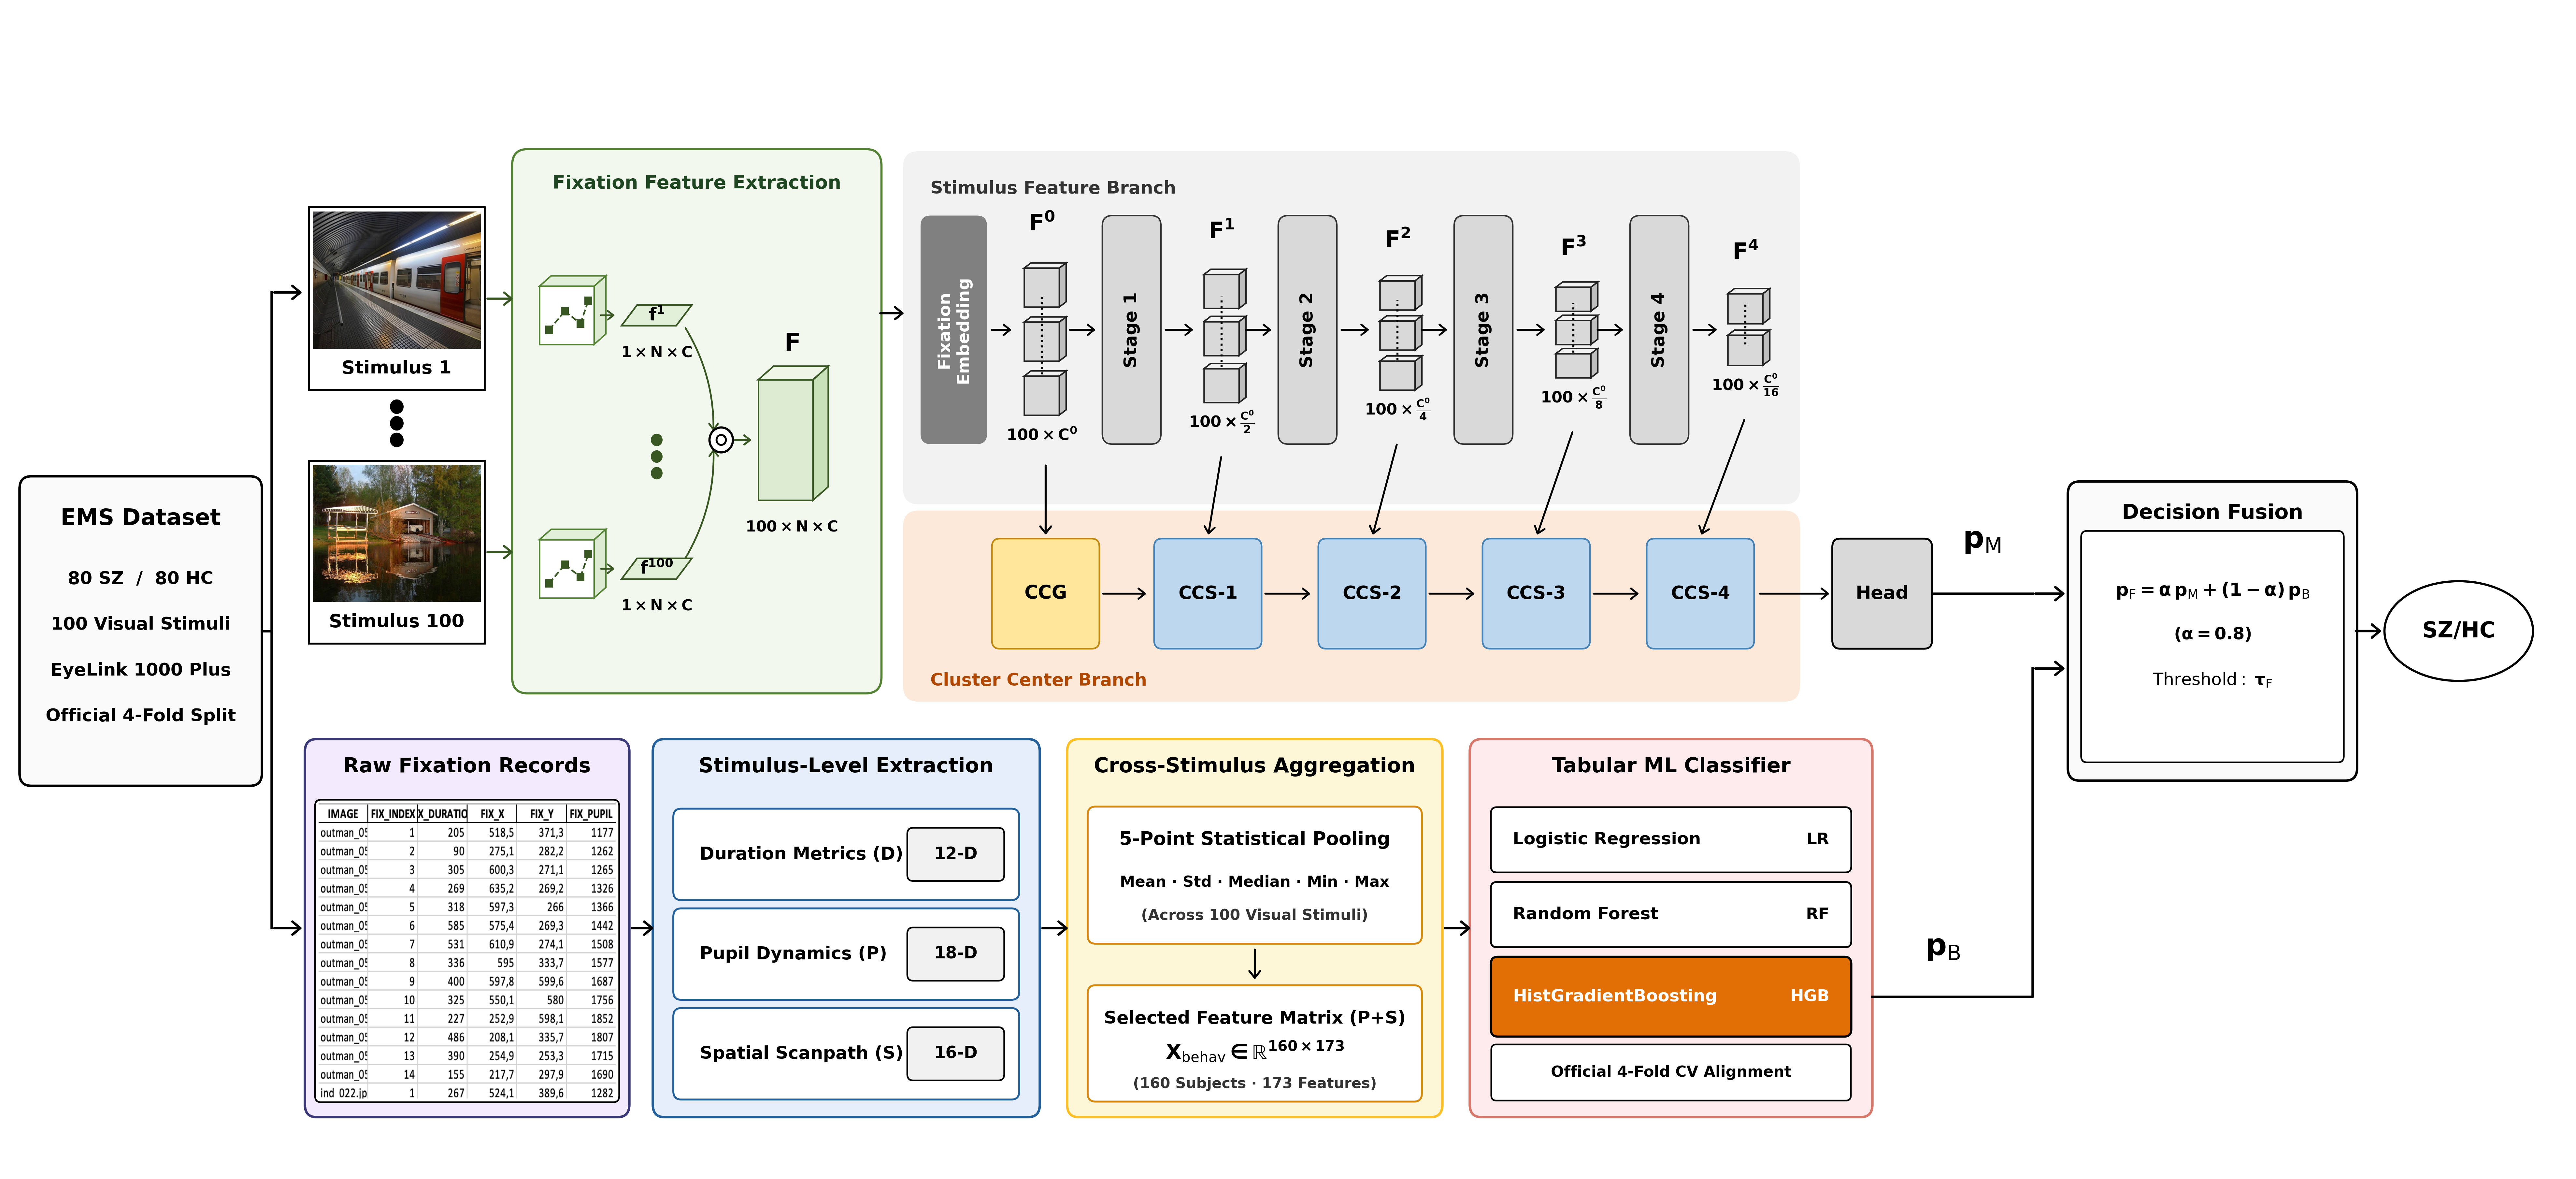
\includegraphics[width=0.99\textwidth]{overall_framework_integrated.png}
\caption{Overview of the proposed behavior-aware multimodal fusion framework BAMF. The upper stimulus-aware path extracts fixation-conditioned feature representations using RINet and processes them through MSNet (comprising SFB and CCB). The lower behavioral path extracts explicit duration ($D$), pupil ($P$), and scanpath ($S$) descriptors for classification via HGB. The final subject-level prediction is obtained via late probability fusion.}
\label{fig:framework}
\end{figure*}

\subsection{Stimulus-Aware MSNet Path}
For stimulus $I_v$, MSNet takes RINet feature vectors at the recorded fixation locations. RINet uses a fully convolutional DenseNet (Densely Connected Convolutional Network) backbone, hierarchical relative-importance enhancement (HRIE) branches, and multi-scale feature merging \cite{song2023rinet}; it is therefore represented with its actual DenseNet-based encoder rather than mislabeled as a ResNet (Residual Network). With $V$ stimuli per subject, the sampled vectors form an input tensor $\mathbf{F}\in\mathbb{R}^{V\times N\times C}$, where the official configuration pads or truncates to $N=14$ fixation locations and uses $C=1056$ channels \cite{song2024ems}. A $1\times1$ fixation-embedding convolution reshapes each stimulus into a compact representation. Four SFB stages then apply channel reduction and self-attention \cite{vaswani2017attention}, allowing each stimulus representation to incorporate information from other stimuli.

In parallel, the CCB first selects a high-density stimulus feature as an initial center through the cluster center generator. At every stage, a cluster center shift module estimates feature density from cosine similarity and updates the center with a mean-shift vector. After the fourth stage, layer normalization, a fully connected layer, and a sigmoid produce the MSNet probability $p_{\mathrm{M}}$. In the main fusion comparison, we reproduce the official pretrained model and do not alter its weights. In the stimulus-set experiments described in Section~\ref{sec:stimulus_design}, the number and identity of stimulus inputs change; consequently, MSNet is trained from scratch for every subset and fold while retaining the original architecture and training protocol.

\subsection{Behavioral Feature Extraction}
For subject $s$ and stimulus $I_j$, the ordered valid fixations are
$\mathcal{Z}_{sj}=\{(d_k,p_k,x_k,y_k)\}_{k=1}^{n_{sj}}$, where $d_k$ is duration, $p_k$ is pupil diameter, and $(x_k,y_k)$ is the fixation position. Records with missing indices or coordinates, or coordinates outside the $1024\times768$ display, are removed. Pupil and duration missingness is retained and handled by training-fold median imputation.

Following the statistical-feature presentation in prior work \cite{vu2026comparative}, we define the common distribution operators for a sequence $v=(v_1,\ldots,v_n)$ as
\begin{equation}
\begin{aligned}
\mathcal{T}(v)=\{&\mu_v,\sigma_v,\operatorname{med}(v),\min(v),\max(v),\\
&Q_{.25}(v),Q_{.75}(v),\operatorname{IQR}(v),\operatorname{CV}(v)\},
\end{aligned}
\label{eq:distribution_features}
\end{equation}
where $\mu_v=n^{-1}\sum_k v_k$ is the mean, $\sigma_v=[n^{-1}\sum_k(v_k-\mu_v)^2]^{1/2}$ is the standard deviation, $\operatorname{IQR}=Q_{.75}-Q_{.25}$ is the interquartile range (IQR), and $\operatorname{CV}=\sigma_v/\mu_v$ is the coefficient of variation (CV) (set to zero when $\mu_v=0$).

The duration group $D$ contains 12 stimulus-level descriptors: $\mathcal{T}(d)$, total duration $\sum_k d_k$, first-fixation duration $d_1$, and the mean of the first $\min(5,n_{sj})$ durations. The pupil group $P$ contains the corresponding distribution, first-fixation, and early-mean descriptors, the missing-pupil ratio, and changes relative to the first and preceding fixations:
\begin{equation}
\Delta_k^{(1)}=p_k-p_1,\qquad \Delta_k^{(s)}=p_{k+1}-p_k,
\label{eq:pupil_changes}
\end{equation}
summarized by their mean, standard deviation, and mean absolute value, yielding 18 descriptors.

For scanpath group $S$, consecutive-fixation amplitude and path length are
\begin{equation}
a_k=\sqrt{(x_{k+1}-x_k)^2+(y_{k+1}-y_k)^2},\qquad L_{sj}=\sum_{k=1}^{n_{sj}-1}a_k.
\label{eq:scanpath}
\end{equation}
We retain fixation count; coordinate means and standard deviations; horizontal, vertical, and rectangular dispersion; mean, standard deviation, and maximum distance to the screen center; $L_{sj}$; and the mean, standard deviation, median, and maximum of $a_k$ (16 descriptors).

Finally, each stimulus-level descriptor is aggregated across the available stimuli for subject $s$ using the mean, standard deviation, median, minimum, and maximum. This yields 60 duration features ($12\times5$), 90 pupil features ($18\times5$), and 80 scanpath features ($16\times5$); three additional statistics—valid-image count, total fixation count, and mean fixations per image—complete the 83-dimensional $S$ group. The resulting feature groups have dimensions of 150 ($D+P$), 143 ($D+S$), 173 ($P+S$), and 233 ($D+P+S$).

\subsection{Behavioral Models and Late Fusion}
We evaluate Logistic Regression (LR), Random Forest (RF), and HistGradientBoosting (HGB). A trained behavioral model $f_{\mathrm{B}}$ estimates
\begin{equation}
p_{\mathrm{B}}=f_{\mathrm{B}}(\mathbf{x}),
\end{equation}
where $\mathbf{x}$ is a subject-level behavioral vector. The final probability is
\begin{equation}
p_{\mathrm{F}}=\alpha p_{\mathrm{M}}+(1-\alpha)p_{\mathrm{B}},\qquad \alpha\in[0,1].
\label{eq:fusion}
\end{equation}
The fusion leaves the two branches independently inspectable. For a target fold, $\alpha$ is selected using predictions from the other three folds, thereby excluding the target fold from its direct weight selection.

\section{Experiments}
\subsection{EMS Dataset and Protocol}
EMS contains 208 subjects: 104 with schizophrenia and 104 HCs \cite{song2024ems}. Each subject free-viewed 100 images for 5 seconds per image. The stimuli include social scenes, natural scenes, synthetic images, and manipulated images. Eye movements were recorded using an EyeLink 1000 Plus at 1000~Hz on a $1024\times768$ display. The released protocol reserves 48 subjects as a hidden test set and divides the remaining 160 balanced subjects into four predefined folds. We follow those folds exactly: one fold is held out for validation and the remaining three train the behavioral model. Table~\ref{tab:dataset} summarizes the data used in this study. Of the 160 training--validation subjects, 148 have processed records for all 100 images and 12 have between 63 and 99 valid images. Rather than discard incomplete subjects, we aggregate over each subject's available images and explicitly retain the valid-image count.

\begin{table}[t]
\caption{Summary of the EMS dataset and evaluation protocol.}
\label{tab:dataset}
\centering
\small
\begin{tabular}{@{}ll@{}}
\toprule
Property & Value \\
\midrule
Participants & 104 SZ + 104 HC \\
Stimuli per participant & 100 images, 5 s each \\
Eye tracker & EyeLink 1000 Plus, 1000 Hz \\
Display & $1024\times768$, 19 inch \\
Train--validation & 160 subjects, four folds \\
Hidden test & 48 subjects (labels withheld) \\
Complete processed records & 148/160 subjects \\
Minimum valid images & 63 \\
\bottomrule
\end{tabular}
\end{table}

\subsection{Experimental Setup}
Missing behavioral values are imputed using medians estimated only from the training folds. LR applies standardization, balanced class weights, the \texttt{liblinear} solver, and at most 3000 iterations. RF uses 500 trees, a minimum leaf size of two, and balanced class weights. HGB uses 300 iterations, a learning rate of 0.03, at most 15 leaf nodes, and $L_2$ regularization of 0.01. The random seed is 42.

The seven behavioral groups are combined with the three classifiers, producing 21 configurations. The MSNet weight is searched on $\alpha\in\{0,0.05,\ldots,1\}$. Area Under the Receiver Operating Characteristic Curve (AUC) is the primary selection criterion, followed by F1-score and accuracy. We report subject-level accuracy (Acc.), sensitivity (Sen.), specificity (Spe.), AUC, precision (Pre.), and F1-score. Following the official EMS code, threshold-dependent metrics use a per-fold Otsu threshold; AUC is threshold independent. All tabulated metrics are unweighted means of the four fold-level values and are expressed as percentages. Best results are bold; second-best results are underlined.

\textcolor{blue}{For a feature-level comparison on the same historical 3/1 folds, each fold's pretrained MSNet supplies a 56-dimensional vector. We concatenate it with 173 pupil--scanpath features and train a 229-input classifier on the other 120 subjects. The classifier retains the structure of the original MSNet head, with one linear layer followed by a sigmoid. One of those three training folds selects the head epoch; we then refit the head on all 120 subjects and score the held-out 40. Behavioral preprocessing is fitted on the corresponding head-training subjects. As in the historical evaluation, threshold-dependent metrics use Otsu on the validation scores without their labels.}

\subsection{Evaluation of proposed model}
Table~\ref{tab:ml_results} reports all 21 behavioral configurations. Duration--pupil LR gives the strongest behavioral-only AUC, while pupil--scanpath HGB is selected for fusion because its errors complement those of MSNet more effectively. Thus, the strongest individual classifier need not produce the strongest fused model.

\begin{table}[t]
\caption{Performance of all behavioral feature--classifier configurations.}
\label{tab:ml_results}
\centering
\footnotesize
\setlength{\tabcolsep}{4.2pt}
\begin{tabular}{llrccccc}
\toprule
Model & Features & Dim. & Acc. & Sen. & Spe. & AUC & F1 \\
\midrule
LR & $D$ & 60 & 75.00 & 66.90 & 82.36 & 81.19 & 72.33 \\
LR & $P$ & 90 & 79.38 & 88.92 & 70.69 & 88.90 & 80.89 \\
LR & $S$ & 83 & 70.62 & 72.61 & 68.06 & 77.23 & 71.17 \\
LR & $D+P$ & 150 & 82.50 & 82.24 & 82.57 & \textbf{90.42} & 82.09 \\
LR & $D+S$ & 143 & 78.13 & 77.50 & 78.12 & 81.78 & 77.89 \\
LR & $P+S$ & 173 & 75.00 & 75.74 & 73.47 & 85.85 & 74.48 \\
LR & $D+P+S$ & 233 & 78.75 & 75.51 & 80.69 & \underline{87.00} & 77.54 \\
\midrule
RF & $D$ & 60 & 69.38 & 76.65 & 62.01 & 77.92 & 71.19 \\
RF & $P$ & 90 & 71.25 & 72.02 & 71.60 & 79.68 & 71.27 \\
RF & $S$ & 83 & 71.88 & 61.82 & 80.14 & 79.00 & 68.19 \\
RF & $D+P$ & 150 & 76.25 & 79.38 & 74.24 & 85.52 & 76.86 \\
RF & $D+S$ & 143 & 73.75 & 69.38 & 77.50 & 79.31 & 71.89 \\
RF & $P+S$ & 173 & 78.12 & 79.72 & 77.64 & \underline{87.81} & 78.12 \\
RF & $D+P+S$ & 233 & 80.00 & 84.26 & 76.04 & \textbf{88.87} & 80.64 \\
\midrule
HGB & $D$ & 60 & 70.62 & 73.64 & 66.32 & 73.48 & 70.38 \\
HGB & $P$ & 90 & 72.50 & 77.93 & 67.50 & 80.83 & 73.67 \\
HGB & $S$ & 83 & 72.50 & 70.62 & 73.40 & 75.50 & 71.57 \\
HGB & $D+P$ & 150 & 75.00 & 77.47 & 71.25 & 84.41 & 74.70 \\
HGB & $D+S$ & 143 & 71.88 & 68.95 & 73.75 & 79.46 & 70.13 \\
HGB & $P+S$ & 173 & 83.12 & 87.24 & 78.96 & \textbf{89.75} & 83.47 \\
HGB & $D+P+S$ & 233 & 76.25 & 84.43 & 67.22 & \underline{87.10} & 77.57 \\
\bottomrule
\end{tabular}
\end{table}

% \subsection{Main Results}
\textcolor{blue}{Table~\ref{tab:main_results} compares the reproduced MSNet, the strongest behavioral-only configuration, feature-level fusion, and the proposed late fusion.} \textcolor{blue}{The historical late fusion uses an MSNet weight of $\alpha=0.8$.} \textcolor{blue}{Late fusion attains the highest AUC, sensitivity, and F1-score and ties feature-level fusion in accuracy.} \textcolor{blue}{Feature-level fusion reaches 92.30\% mean AUC, above MSNet's 89.72\% but below late fusion's 95.03\%; its accuracy is 84.38\%. Relative to MSNet, late fusion raises mean AUC by 5.30 percentage points, reduces false negatives, and lowers specificity by 3.47 points. The accuracy gain corresponds to two additional correct decisions among 160 subjects. The 21 feature--classifier configurations and fusion weights were compared on the same four development folds, so the reported performance of the selected configuration may be optimistic. The feature-level comparison is also internal development validation.}


% We verified specificity as $\mathrm{TN}/(\mathrm{TN}+\mathrm{FP})$ within each fold before macro-averaging; the result therefore reflects a genuine sensitivity--specificity trade-off rather than a transcription error.

\begin{table}[t]
\caption{\textcolor{blue}{Mean subject-level performance over the four EMS development folds (\%).}}
\label{tab:main_results}
\centering
\footnotesize
\setlength{\tabcolsep}{3pt}
\begin{tabular}{@{}llrrrrr@{}}
\toprule
Method & Configuration & Acc. & Sen. & Spe. & AUC &  F1 \\
\midrule
MSNet & Pretrained & \textcolor{blue}{\underline{83.13}} & 80.51 & \textbf{87.08} & 89.72 & \textcolor{blue}{82.44} \\
Behavioral & $D+P$, LR & 82.50 & \textcolor{blue}{82.24} & 82.57 & \textcolor{blue}{90.42} & 82.09 \\
\textcolor{blue}{Early fusion} & \textcolor{blue}{229-d linear} & \textcolor{blue}{\textbf{84.38}} & \textcolor{blue}{\underline{82.47}} & \textcolor{blue}{\underline{86.04}} & \textcolor{blue}{\underline{92.30}} & \textcolor{blue}{\underline{83.95}} \\
BAMF (ours) & $P+S$, HGB & \textbf{84.38} & \textbf{84.63} & \textcolor{blue}{83.61} & \textbf{95.03} &  \textbf{84.05} \\
\bottomrule
\end{tabular}
\end{table}

To place the result in the official benchmark, Table~\ref{tab:benchmark} lists all published EMS validation baselines \cite{song2024ems}, spanning classical feature-based methods with Support Vector Machine (SVM), Quadratic Discriminant Analysis (QDA), Bayesian (BYS), and RF classifiers, as well as deep sequence models based on Long Short-Term Memory (LSTM) and Gated Recurrent Unit (GRU) networks. Our reproduced MSNet numbers match the official values, providing a consistency check. The proposed BAMF method produces the best validation AUC among the compared methods. 

\begin{table}[t]
\caption{Comparison with the official EMS validation benchmark \cite{song2024ems}. Baselines represent published statistical and deep learning models (SVM, QDA, BYS, RF, LSTM, GRU) evaluated on the four-fold validation set.} 
\label{tab:benchmark}
\centering
\footnotesize
\setlength{\tabcolsep}{7.0pt}
\begin{tabular}{lccccc}
\toprule
Method & Acc. & Sen. & Spe. & AUC & F1 \\
\midrule
EDB--SVM & 73.13 & 71.56 & 73.96 & 80.86 & 71.95 \\
EDB--QDA & 70.63 & 60.26 & 79.93 & 72.05 & 66.38 \\
EDB--BYS & 70.00 & 60.65 & 77.85 & 79.87 & 65.10 \\
ESR--SVM & 79.38 & 79.46 & 78.47 & 84.98 & 78.89 \\
ESR--RF & 76.25 & 75.40 & 76.39 & 85.21 & 75.38 \\
IAS & 75.63 & 76.34 & 75.00 & 81.80 & 75.72 \\
LVA & 81.88 & 77.66 & 85.85 & 89.87 & 80.96 \\
DDB--DoF & 72.50 & 78.72 & 67.27 & 76.45 & 74.46 \\
DDB & 73.13 & 78.66 & 68.73 & 77.72 & 75.12 \\
DVP & 78.75 & 75.48 & 80.56 & 85.16 & 77.69 \\
GPI--LSTM & 71.25 & 68.81 & 74.24 & 79.53 & 69.47 \\
GPI--GRU & 70.63 & 70.45 & 71.88 & 77.98 & 69.83 \\
MSNet & \underline{83.13} & \underline{80.51} & \textbf{87.08} & \underline{89.72} & \underline{82.44} \\
\midrule
BAMF (ours) & \textbf{84.38} & \textbf{84.63} & \underline{83.61} & \textbf{95.03} & \textbf{84.05} \\
\bottomrule
\end{tabular}
\end{table}

\subsection{Fusion-Weight and Fold-Wise Analysis}
Figure~\ref{fig:alpha_curve} analyzes the selected pupil--scanpath HGB branch over the fusion grid. Performance improves as the behavioral and deep probabilities are combined and peaks at $\alpha=0.8$. The point $\alpha=0$ refers specifically to pupil--scanpath HGB, not to the duration--pupil LR model in Table~\ref{tab:main_results}. Fusion improves AUC in every fold: from 89.65\% to 97.98\% on Set\_0, 89.84\% to 91.93\% on Set\_1, 89.75\% to 95.75\% on Set\_2, and 89.65\% to 94.44\% on Set\_3. The respective gains are 8.33, 2.08, 6.00, and 4.80 percentage points.

\textcolor{blue}{With the pretrained MSNet scores held constant, rerunning the pupil--scanpath HGB branch at seeds 42, 17, and 2026 yielded identical subject-level predictions and zero sample variance in all reported metrics. The mean validation AUC was 95.03\%.}

\begin{figure}[t]
\centering
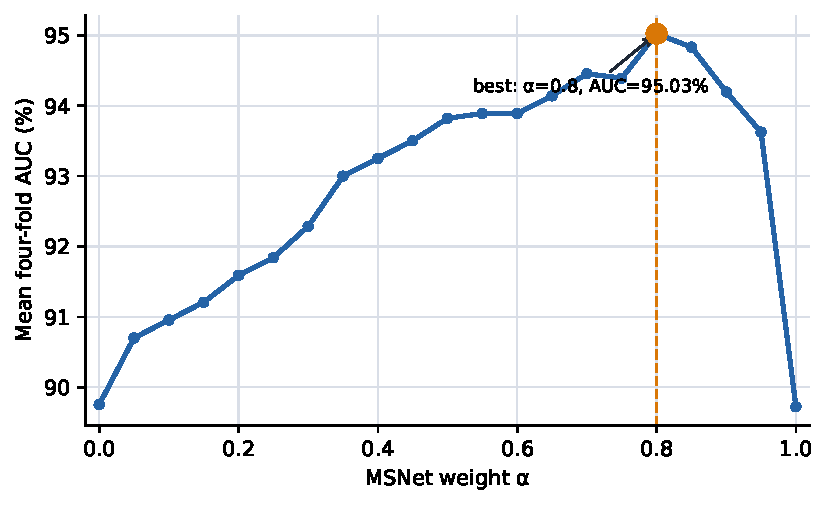
\includegraphics[width=0.8\columnwidth]{alpha_grid_auc_curve_revised.pdf}
\caption{Mean four-fold AUC versus MSNet weight $\alpha$ for the selected pupil--scanpath HGB fusion.}
\label{fig:alpha_curve}
\end{figure}

\subsection{\textcolor{blue}{Separated 2/1/1 Validation}}
\textcolor{blue}{We rotate the four EMS folds through a 2/1/1 protocol to separate tuning from evaluation. For each evaluation fold, the next fold cyclically serves as the tuning fold. The remaining two folds (80 subjects) train MSNet and the behavioral models. We train MSNet from scratch for 50 epochs with batch size 8, AdamW, and a cosine learning-rate schedule with five warmup epochs. Following the released EMS training code, we select the checkpoint that maximizes the sum of AUC and Otsu-based accuracy on the 40 tuning subjects and reload the best weights before each subsequent epoch. The selected checkpoint is shared by the MSNet baseline, early fusion, and late fusion. All model and threshold choices are made before scoring the 40 evaluation subjects. We report unweighted means over the four evaluation folds.}

\textcolor{blue}{For feature-level fusion, we freeze the same selected MSNet encoder used by the MSNet baseline and late fusion. The 56-dimensional vector before the original classification head is concatenated with the 173 pupil--scanpath features. Median imputation and scaling are fitted on the 80 training subjects. The resulting 229-dimensional vector is passed through a linear classifier followed by a sigmoid. We fit the classifier on the training subjects, select its epoch by AUC on the tuning fold, and estimate an Otsu threshold from the tuning scores. Early fusion attains 83.93\% mean AUC under this protocol.}

\begin{table}[t]
\color{blue}
\caption{\textcolor{blue}{Separated 2/1/1 validation with MSNet checkpoints selected on the tuning fold (\%). AUC SD is the sample standard deviation across the four evaluation folds.}}
\label{tab:separated_validation}
\centering
\footnotesize
\setlength{\tabcolsep}{2.8pt}
\begin{tabular}{lrrrrrr}
\toprule
Method & Acc. & Sen. & Spe. & AUC & AUC SD & F1 \\
\midrule
MSNet (80 train) & 68.13 & 69.01 & 68.47 & 78.10 & 6.10 & 66.93 \\
Late fusion & 76.25 & 78.21 & 73.68 & 84.69 & 1.44 & 76.22 \\
Early fusion & 70.63 & 65.99 & 74.38 & 83.93 & 3.70 & 68.13 \\
\bottomrule
\end{tabular}
\end{table}

\textcolor{blue}{For late fusion, we fit pupil--scanpath HGB on the 80 training subjects and select $\alpha$ from $\{0,0.05,\ldots,1\}$ on the tuning fold. We rank the fused scores by AUC, followed by F1-score and accuracy, and estimate the Otsu threshold on the tuning fold. The weights for Set\_0 through Set\_3 are 0.05, 0.20, 0.70, and 0.70. Early and late fusion improve mean AUC over the shared MSNet baseline by 5.83 and 6.59 percentage points, respectively. The 2/1/1 results and the historical 95.03\% AUC use different training-set sizes and checkpoint rules.}

\subsection{Stimulus-Set Design Experiments}
\label{sec:stimulus_design}
After selecting the best fusion configuration, we keep the behavioral representation ($P+S$), HGB hyperparameters, and fusion weight ($\alpha=0.8$) fixed and vary only the stimulus set. For each reduced set, the behavioral descriptors are recomputed exclusively from its selected images and MSNet is retrained from scratch for each of the four official subject folds. Thus, there is no leakage from excluded stimuli. The full 100-image result in Table~\ref{tab:stimulus_count} uses the official pretrained MSNet and serves as the reference. All metrics retain the same fold-wise Otsu thresholding and macro-averaging protocol as the main experiment.
\begin{figure*}[htbp]
\centering
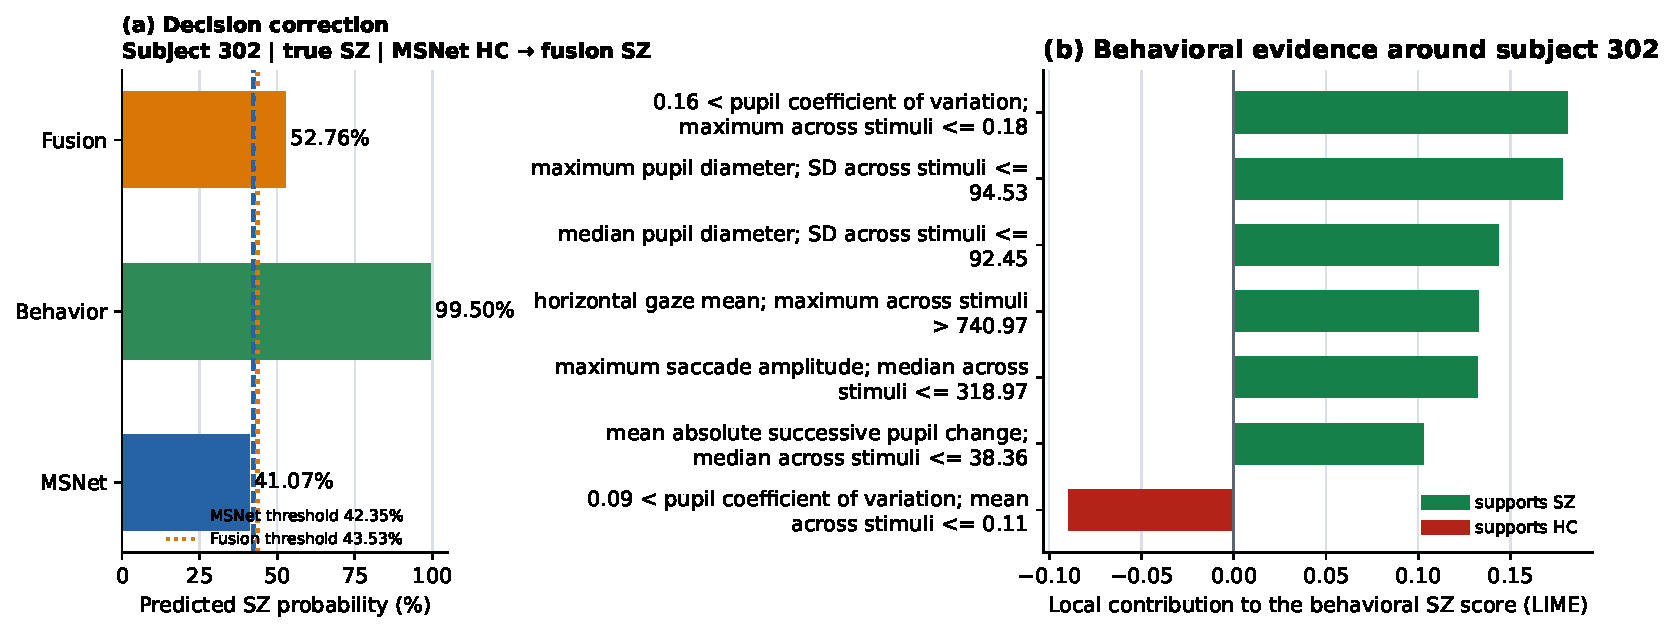
\includegraphics[width=0.8\textwidth]{xai_subject_302.pdf}
\caption{Explainable decision correction for subject 302 (ground truth: SZ). (a) The behavioral branch raises the weighted fusion score across the fold-specific decision boundary. (b) LIME contributions around the behavioral HGB prediction; green conditions support SZ and red conditions support HC.}
\label{fig:xai_case}
\end{figure*}
\subsubsection{Category-specific analysis}
The first experiment partitions the 100 EMS stimuli into manipulated images (32), natural scenes (31), social scenes (22), and synthetic images (15). Table~\ref{tab:category_results} shows that natural scenes attain the highest category-specific AUC (91.29\%) and sensitivity (86.08\%). Manipulated images are a close second in AUC (91.00\%), while providing the highest specificity (80.00\%) and the smallest cross-fold AUC standard deviation (3.92 points). Synthetic images give the lowest values across most metrics. The 0.29-point AUC difference between natural and manipulated images is too small to support a strong claim of category superiority, particularly because the category sizes are unequal. The experiment therefore suggests that natural and manipulated content are promising candidates for prioritization, but it does not isolate category semantics from stimulus count.

\begin{table}[t]
\caption{Performance (\%) of BAMF when trained and tested on specific categories of stimuli.}
\label{tab:category_results}
\centering
\small
\setlength{\tabcolsep}{5.2pt}
\begin{tabular}{@{}lrrrrrr@{}}
\toprule
Category & Images & Acc. & Sen. & Spe. & AUC & F1 \\
\midrule
Manipulated & 32 & 79.38 & 77.36 & \underline{80.00} & 91.00 & 77.75 \\
Natural & 31 & \underline{81.25} & \textbf{86.08} & 74.65 & \underline{91.29} & \underline{80.88} \\
Social & 22 & 79.38 & 81.82 & 76.81 & 88.87 & 79.28 \\
Synthetic & 15 & 72.50 & 71.45 & 72.64 & 84.34 & 71.47 \\
All & 100 & \textbf{84.38} & \underline{84.63} & \textbf{83.61} & \textbf{95.03} & \textbf{84.05} \\
\bottomrule
\end{tabular}
\end{table}


\subsubsection{Balanced stimulus-count analysis}
The second experiment constructs three nested subsets with seed 42: $S_{20}\subset S_{40}\subset S_{60}$. They contain respectively 5, 10, and 15 images from each category, thereby controlling category balance while varying stimulus count. Table~\ref{tab:stimulus_count} reveals a clear AUC increase from 83.67\% at 20 images to 88.15\% at 40 and 91.70\% at 60. The 60-image subset is the strongest reduced design: compared with all 100 images, its accuracy is only 0.63 points lower, its F1-score is 0.03 points higher, and its sensitivity is 4.89 points higher. However, its AUC remains 3.32 points lower and its specificity is 6.18 points lower. Hence, 60 balanced images offer a promising 40\% reduction in the number of stimuli, but cannot yet be called statistically equivalent to the full set.

\begin{table}[t]
\caption{Performance (\%) of BAMF when trained and tested across various sizes of stimulus sets.}
\label{tab:stimulus_count}
\centering
\small
\setlength{\tabcolsep}{5.2pt}
\begin{tabular}{lrrrrrr}
\toprule
Set & Per category & Acc. & Sen. & Spe. & AUC & F1 \\
\midrule
$S_{20}$ & 5 & 75.63 & 76.93 & 72.64 & 83.67 & 74.47 \\
$S_{40}$ & 10 & 75.63 & \underline{84.83} & 65.76 & 88.15 & 77.22 \\
$S_{60}$ & 15 & \underline{83.75} & \textbf{89.52} & \underline{77.43} & \underline{91.70} & \textbf{84.09} \\
$S_{100}$ & unbalanced & \textbf{84.38} & 84.63 & \textbf{83.61} & \textbf{95.03} & \underline{84.05} \\
\bottomrule
\end{tabular}
\end{table}

\subsection{Explainable Case and Error Analysis}
Figure~\ref{fig:xai_case} explains a representative recovered SZ case. For subject 302, the MSNet probability of 41.07\% is below its Set\_0 threshold of 42.35\%, producing an HC decision. The pupil--scanpath HGB branch assigns 99.50\% SZ probability; with $\alpha=0.8$, fusion reaches 52.76\%, above its 43.53\% threshold. A model-agnostic Local Interpretable Model-agnostic Explanations (LIME) explanation is fitted locally around this subject using the same training folds and exact HGB pipeline. It identifies the behavioral conditions that support or oppose the HGB SZ score; the explanation is descriptive rather than causal.

\section{Conclusion}
We presented BAMF, a behavior-aware late-fusion framework for eye-movement-based schizophrenia recognition. The method complements the stimulus-aware MSNet probability with explicit fixation-duration, pupil-response, and scanpath statistics. Under the official EMS four-fold validation protocol, the proposed pupil--scanpath HGB fusion increases mean AUC from 89.72\% to 95.03\% and improves AUC in all four folds. Pooled errors and the Explainable Artificial Intelligence (XAI) case study show that the gain primarily arises from recovering false-negative SZ cases, while also revealing a small increase in HC false positives. With this configuration fixed, natural scenes produce the highest observed category-specific AUC, closely followed by manipulated images, and a balanced 60-image subset nearly preserves full-set accuracy and F1-score while reducing the stimulus count by 40\%. \textcolor{blue}{Under separated 2/1/1 validation, early fusion and late fusion attain 83.93\% and 84.69\% mean AUC, respectively, compared with 78.10\% for MSNet trained on the same 80 subjects in each rotation. The selected late-fusion weights vary across folds. Identical predictions across three seeds of the fixed pretrained-MSNet branch do not establish population-level confidence.} These findings indicate that deep stimulus representations and interpretable behavioral summaries contain complementary information and that stimulus selection may improve acquisition efficiency. Repeated stimulus sampling, a controlled 100-image training reference, external validation, and stricter nested model selection are necessary before the proposed dataset-design guidance or clinical use can be considered definitive.

\bibliographystyle{IEEEtran}
\bibliography{references}

\end{document}
